%-----------------------------------------------------------------------------
%
%               Template for sigplanconf LaTeX Class
%
% Name:         sigplanconf-template.tex
%
% Purpose:      A template for sigplanconf.cls, which is a LaTeX 2e class
%               file for SIGPLAN conference proceedings.
%
% Guide:        Refer to "Author's Guide to the ACM SIGPLAN Class,"
%               sigplanconf-guide.pdf
%
% Author:       Paul C. Anagnostopoulos
%               Windfall Software
%               978 371-2316
%               paul@windfall.com
%
% Created:      15 February 2005
%
%-----------------------------------------------------------------------------


\documentclass[10pt]{sigplanconf}

% The following \documentclass options may be useful:

% preprint      Remove this option only once the paper is in final form.
% 10pt          To set in 10-point type instead of 9-point.
% 11pt          To set in 11-point type instead of 9-point.
% authoryear    To obtain author/year citation style instead of numeric.

\usepackage{amsmath}
\usepackage{graphicx}
\usepackage[space]{grffile}
\usepackage{latexsym}
\usepackage{amsfonts,amsmath,amssymb}
\usepackage{url}
\usepackage[utf8]{inputenc}
\usepackage{hyperref}
\hypersetup{colorlinks=false,pdfborder={0 0 0}}
\usepackage{textcomp}
\usepackage{longtable}
\usepackage{multirow,booktabs}

\newcommand{\noauthorea}{}
% http://ctan.mirror.garr.it/mirrors/CTAN/info/symbols/comprehensive/symbols-a4.pdf
% http://detexify.kirelabs.org/classify.html

\usepackage{color}
\usepackage{listings}

% clever references
\ifdefined\noauthorea
\usepackage{cleveref} 
\AtBeginDocument{\renewcommand{\ref}[1]{\Cref{#1}}}
\AtBeginDocument{\renewcommand{\eqref}[1]{\Cref{#1}}}
\fi

% commands
\ifdefined\noauthorea
\newcommand{\ifauthorea}[2]{#2}
\else
\newcommand{\ifauthorea}[2]{#1}
\fi

\newcommand{\mynote}[1]{\medskip\noindent{\small[{\bf Note:} {\em #1}]}}

% macros
\newcommand{\tinyvm}{{\sc Anony}}
\newcommand{\feval}{{\tt feval}}
\newcommand{\fbase}{\textsf{f}}
\newcommand{\fvariant}{\textsf{f'}}
\newcommand{\fosrfrom}{$\textsf{f}_{\textsf{OSRfrom}}$}
\newcommand{\fosrto}{$\textsf{f}\textsf{'}_{\textsf{OSRto}}$}

% theorems
\newtheorem{theorem}{Theorem}
\newtheorem{lemma}{Lemma}
\newtheorem{corollary}{Corollary}
\newtheorem{definition}{Definition}
\newtheorem{property}{Property}
\newtheorem{example}{Example}

% settings
\lstset {
%  backgroundcolor=\color{white},   % choose the background color; you must add \usepackage{color} or \usepackage{xcolor}
%  basicstyle=\footnotesize,        % the size of the fonts that are used for the code
%  breakatwhitespace=false,         % sets if automatic breaks should only happen at whitespace
%  breaklines=true,                 % sets automatic line breaking
%  captionpos=b,                    % sets the caption-position to bottom
%  commentstyle=\color{mygreen},    % comment style
%  deletekeywords={...},            % if you want to delete keywords from the given language
%  escapeinside={\%*}{*)},          % if you want to add LaTeX within your code
%  extendedchars=true,              % lets you use non-ASCII characters; for 8-bits encodings only, does not work with UTF-8
%  frame=single,	                   % adds a frame around the code
  keepspaces=true,                 % keeps spaces in text, useful for keeping indentation of code (possibly needs columns=flexible)
  keywordstyle=\tt\bf,       % keyword style
%  language=Octave,                 % the language of the code
%  otherkeywords={},            % if you want to add more keywords to the set
  numbers=left,                    % where to put the line-numbers; possible values are (none, left, right)
  numbersep=5pt,                   % how far the line-numbers are from the code
%  numberstyle=\tiny\color{mygray}, % the style that is used for the line-numbers
%  rulecolor=\color{black},         % if not set, the frame-color may be changed on line-breaks within not-black text (e.g. comments (green here))
  showspaces=false,                % show spaces everywhere adding particular underscores; it overrides 'showstringspaces'
  showstringspaces=false,          % underline spaces within strings only
  showtabs=false,                  % show tabs within strings adding particular underscores
  stepnumber=1,                    % the step between two line-numbers. If it's 1, each line will be numbered
%  stringstyle=\color{mymauve},     % string literal style
  tabsize=4,	                   % sets default tabsize to 2 spaces
%  title=\lstname,                   % show the filename of files included with \lstinputlisting; also try caption instead of title
  basicstyle=\ttfamily,
  morekeywords={in,out,if},
  xleftmargin=20pt
}

  
  
  
  
  
  
  
  
  

\begin{document}

\special{papersize=8.5in,11in}
\setlength{\pdfpageheight}{\paperheight}
\setlength{\pdfpagewidth}{\paperwidth}

\conferenceinfo{CONF 'yy}{Month d--d, 20yy, City, ST, Country} 
\copyrightyear{20yy} 
\copyrightdata{978-1-nnnn-nnnn-n/yy/mm} 
\doi{nnnnnnn.nnnnnnn}

% Uncomment one of the following two, if you are not going for the 
% traditional copyright transfer agreement.

%\exclusivelicense                % ACM gets exclusive license to publish, 
                                  % you retain copyright

%\permissiontopublish             % ACM gets nonexclusive license to publish
                                  % (paid open-access papers, 
                                  % short abstracts)

\titlebanner{banner above paper title}        % These are ignored unless
\preprintfooter{short description of paper}   % 'preprint' option specified.

\newcommand{\anon}{$\bullet\bullet\bullet\bullet\bullet$}

\title{Platform agnostic On-Stack Replacement in LLVM
  }
%\subtitle{Subtitle Text, if any}

\authorinfo{\anon\ \and \anon}
           {\anon} % affil
           {\anon} % email

\maketitle

\begin{abstract}
% !TEX root = article.tex

On-Stack Replacement (OSR) is a technique for dynamically diverting execution between different versions of a function at run time.
%suspending the execution of a function and continuing with a different version of the code. 
OSR is typically used in virtual machines to interrupt a long-running function and recompile it at a higher optimization level, or to replace it with a different one when a speculative assumption made during its compilation no longer holds.

In this paper we present a framework for OSR that introduces novel ideas and combines features of extant techniques that no previous solution provided simultaneously. New features include OSR with compensation code to adjust the program state during a transition and the ability to fire an OSR from arbitrary locations in the code. Our approach is platform-independent as the OSR machinery is entirely encoded at a compiler's intermediate representation level.

%Compared to extant OSR techniques, our approach is platform-independent as transitions are encoded entirely at the Intermediate Representation (IR) level; it supports OSR-point insertion at arbitrary locations in a function, 

%and it allows a function version reached via OSR to fire an OSR itself, either to a more optimized version or to a less optimized one from which it was derived.

We implement and evaluate our technique in the LLVM compiler infrastructure, which is gaining popularity as Just-In-Time (JIT) compiler in virtual machines for dynamic languages such as Javascript, MATLAB, Python, and Ruby. As a case study of our approach, we show how to improve the state of the art in the optimization of the \feval\ instruction, a performance-critical construct of the MATLAB language.

%We also present a case study on the integration of our technique in the McVM virtual machine for MATLAB, showing significant speedups from the run-time optimization of a typical construct of the language.
  
  
  
  
  
  
  
  
  
\end{abstract}

\category{D.3}{Processors}{Compilers}

% general terms are not compulsory anymore, 
% you may leave them out
%\terms
%term1, term2

\keywords
On-stack replacement, code optimization, LLVM

\section{Introduction}
\label{se:intro}

[...]

% !TEX root = article.tex

\ifdefined\noauthorea
\begin{figure}[t]
\begin{center}
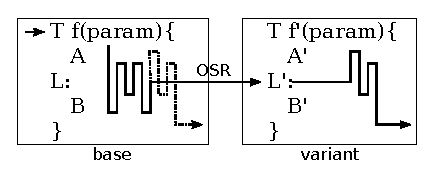
\includegraphics[width=0.6\columnwidth]{figures/overview-osr/overview-osr.eps}
\caption{\protect\label{fig:osr-dynamics} On-stack replacement dynamics: control is transferred via OSR from a point \textsf{L} of a base function \textsf{f} to a point \textsf{L'} in a variant \textsf{f'} of \textsf{f}.
  
  
  
  
  
  
  
  }
\end{center}
\end{figure}
\fi

\section{Overview}
\label{se:overview}

The key to platform independence in our work is to express the entire OSR machinery at intermediate code representation level, without resorting to machine-level code manipulation or special intrinsics of the intermediate language. %Before describing how this is achieved in LLVM, we provide an overview of our approach.

%\subsection{Overview}
%\label{ss:overview}

Consider the generic OSR scenario shown in \myfigure\ref{fi:osr-dynamics}. A base function \fbase\ is executed and it can either terminate normally (dashed lines), or an OSR event may transfer control to a variant \fvariant. The decision of whether an OSR should be fired at a given point \osrpoint\ of \fbase\ is based on an {\em OSR condition}. A typical example in JIT-based virtual machines is a profile counter reaching a certain hotness threshold, which indicates that \fbase\ is taking longer than expected and is worth optimizing. Another example is a guard testing whether \fbase\ has become unsafe and execution needs to fall back to a safe version \fvariant. This scenario includes deoptimization of functions generated with aggressive speculative optimizations. 

Classical OSR implementations adjust the stack so that execution can continue in \fvariant\ with the current frame \cite{chambers1992design}. This requires manipulating the program state at machine code level and is highly ABI- and compiler-dependent. A simpler approach, which we follow in this article, consists of creating a new frame every time an OSR is fired, essentially regarding an OSR transition as a function call~\cite{Lameed_2013,webkit14}. 

Our implementation targets two general scenarios: 1) {\em resolved OSR}: \fvariant\ is known before executing \fbase\ as in the deoptimization example discussed above; 2) {\em open OSR}: \fvariant\ is generated when the OSR is fired, supporting deferred compilation strategies. In both cases, \fbase\ is instrumented before its execution to incorporate the OSR machinery. We call such OSR-instrumented version \fosrfrom.

\ifdefined\noauthorea
\begin{figure}[t]
\begin{center}
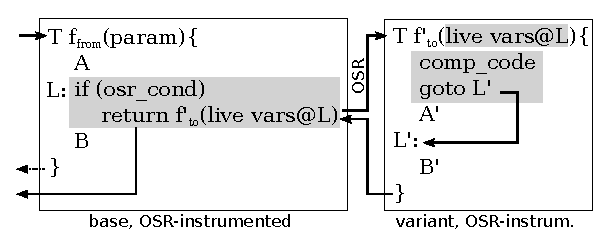
\includegraphics[width=0.7\columnwidth]{figures/overview-osr-final/overview-osr-final.eps}
\caption{\protect\label{fi:overview-osr-final} OSR-instrumented functions with resolved OSR call.}
\end{center}
\end{figure}
\fi

In the resolved OSR scenario (see \myfigure\ref{fi:overview-osr-final}), instrumentation consists of adding a check of the OSR condition and, if it is satisfied, a tail call that fires the OSR. The called function is an instrumented version of \fvariant, which we call \fosrto. The assumption is that \fosrto\ produces the same side-effects and return value that one would obtain by \fbase\ if no OSR was performed. Differently from \fvariant, \fosrto\ takes as input all live variables of \fbase\ at \osrpoint, executes an optional compensation code to fix the computation state ({\tt comp\_code}), and then jumps to a point \textsf{L'} from which execution can continue. The OSR practice often makes the conservative assumption that execution can always continue with the very same program state as the base function. However, this assumption may reduce the number of points where sound OSR transitions can be fired. Supporting compensation code in our framework adds flexibility, allowing OSR transitions to happen at arbitrary places in the base function.

\ifdefined\noauthorea
\begin{figure}[h!]
\begin{center}
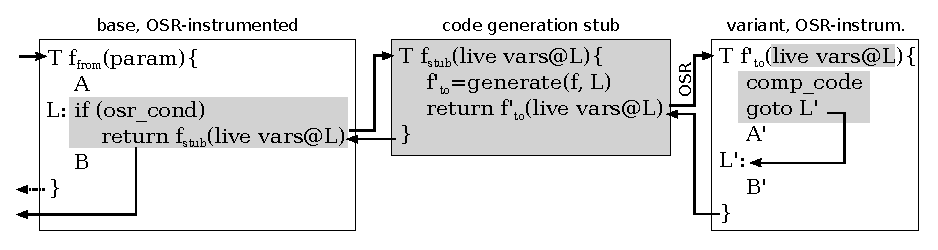
\includegraphics[width=1.0\columnwidth]{figures/overview-osr-open/overview-osr-open.eps}
\caption{\protect\label{fi:overview-osr-open} Functions of \ifauthorea{Figure~}{}\ref{fig:osr-dynamics} instrumented for open OSR.
  
  }
\end{center}
\end{figure}
\fi

The open OSR scenario is similar, with one main difference (see \myfigure\ref{fi:overview-osr-open}): instead of calling \fosrto\ directly, \fosrfrom\ calls a stub function \fstub, which first creates \fosrto\ and then calls it. Function \fosrto\ is generated by a function {\tt gen} that takes the base function \fbase\ and the OSR point \osrpoint\ as input. The reason for having a stub in the open OSR scenario, rather than directly instrumenting \fbase\ with the code generation machinery, is to minimize the extra code injected into \fbase. Indeed, instrumentation may interfere with optimizations, e.g., by increasing register pressure and altering code layout and instruction cache behavior.


\paragraph{Discussion.}
Instrumenting functions for OSR at a higher level than machine code yields several benefits: 
\begin{enumerate}
\item {\em Platform independence}: the OSR instrumentation code is lowered to native code by the compiler backend, which handles the details of the target ABI; 
\item {\em Global optimizations}: lowering OSR instrumentation code along with the application code can generate faster code than local binary instrumentation. For instance, dead code elimination can suppress from \fosrto\ portions of code that would no longer be needed when jumping to the landing pad \textsf{L'}, producing smaller code and enabling better register allocation and instruction scheduling.
\item {\em Debugging and Profiling}: preserving ABI conventions in the native code versions of \fosrfrom, \fstub, and \fosrto\ helps debuggers and profilers to more precisely locate the current execution context and collect more informative data.
%avoiding low-lever tampering with stack frames can more easily preserve ABI calling conventions
\item {\em Abstraction}: the approach is amenable to a clean instrumentation API that abstracts the OSR implementation details, allowing a front-end to focus on where to insert OSR points independently of the final target architecture.
%by analyzing code at an intermediate representation level.
\end{enumerate}

\noindent A natural question is whether encoding OSR at a higher level of abstraction can result in poorer performance than binary code approaches. We address this issue in \mysection\ref{se:osr-llvm}, where we analyze the OSR machine code generated for an x86-64 target, and in \mysection\ref{se:experiments}, where OSR performance is measured on classical benchmarks.

  
  
  
  
  
  
  
  
  
  
  
  
  
  
  
  
  
  
  
  
  
  
  
  
  
  
  
  
  
  
  
  
  
  
  
  
  
  
  
  
  
  
  
  
  
  
  
  
  
  
  
  
  
  
  
  
  
  
  
  
  
  
  
  
  
  
  
  
  
  
  
  
  
  
  
  
  
  
  
  
  
  
  
  
  
  
  
  
% !TEX root = article.tex

\section{OSR in LLVM}
\label{se:osr-llvm}

% ====> The following text goes in the artifact
% In this section we discuss our implementation of the approach described in \mysection\ref{se:overview} in \tinyvm, a proof-of-concept virtual machine we developed as a playground to exercise our OSR techniques. TinyVM is based on LLVM's MCJIT compiler and supports interactive invocation of LLVM IR functions either generated at run-time or loaded from disk. The main design goal behind TinyVM is the creation of an interactive environment for IR manipulation and JIT-compilation of functions: for instance, it allows the user to insert OSR points in loaded functions, run optimization passes on them or display their CFGs, repeatedly invoke a function for a specified amount of times and so on. TinyVM supports dynamic library loading and linking, and comes with a helper component for MCJIT that simplifies tasks such as handling multiple IR modules, symbol resolution in presence of multiple versions of a function, and tracking native code and other machine-level generated object such as Stackmaps.

\ifdefined\noauthorea
\begin{figure}[t]
\begin{center}
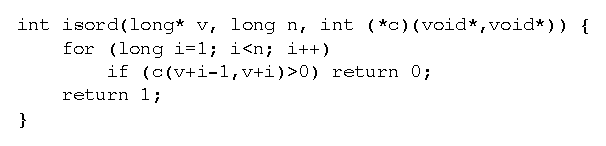
\includegraphics[width=0.9\columnwidth]{figures/isord-example/isord.eps}
\caption{\protect\label{fig:isordfrom} OSR instrumentation of base function in LLVM IR (in grey). The OSR is fired at the beginning of the loop body after 1000 iterations.
}
\end{center}
\end{figure}
\fi

%\subsection{Example}
In this section we discuss one possible embodiment of the OSR approach of \mysection\ref{se:overview} in LLVM. Our discussion is based on a simple running example that illustrates a profile-driven optimization scenario. We start from a simple base function ({\tt isord}) that checks whether an array of numbers is ordered according to some criterion specified by a comparator (see \myfigure\ref{fi:isord-example}). Our goal is to instrument {\tt isord} so that, whenever the number of loop iterations exceeds a certain threshold, control is dynamically diverted to a faster version generated on the fly by inlining the comparator. 

The IR code shown in this section\footnote{Virtual register names and labels in the LLVM-produced IR code shown in this paper have been refactored to make the code more readable.} has been generated with \clang\ and instrumented with \osrkit, a library we prototyped to help VM builders deploy OSR in LLVM. \osrkit\ provides a number of useful abstractions that include open and resolved OSR instrumentation of IR base functions without breaking the SSA form, liveness analysis, generation of OSR continuation functions, and mapping of LLVM values between different versions of a program along with compensation code generation\footnote{The accompanying artifact allows the interested reader to get acquainted with \osrkit\ and repeat the sample scenario described in this section.}.

%To explain how the OSR approach of \mysection\ref{se:overview} can be implemented in LLVM, we consider the simple example of \myfigure\ref{fi:isord-example}. Function {\tt isord} checks whether an array of numbers is ordered according to some criterion specified by a comparator.

\ifdefined\noauthorea
\begin{figure}[t]
\begin{center}
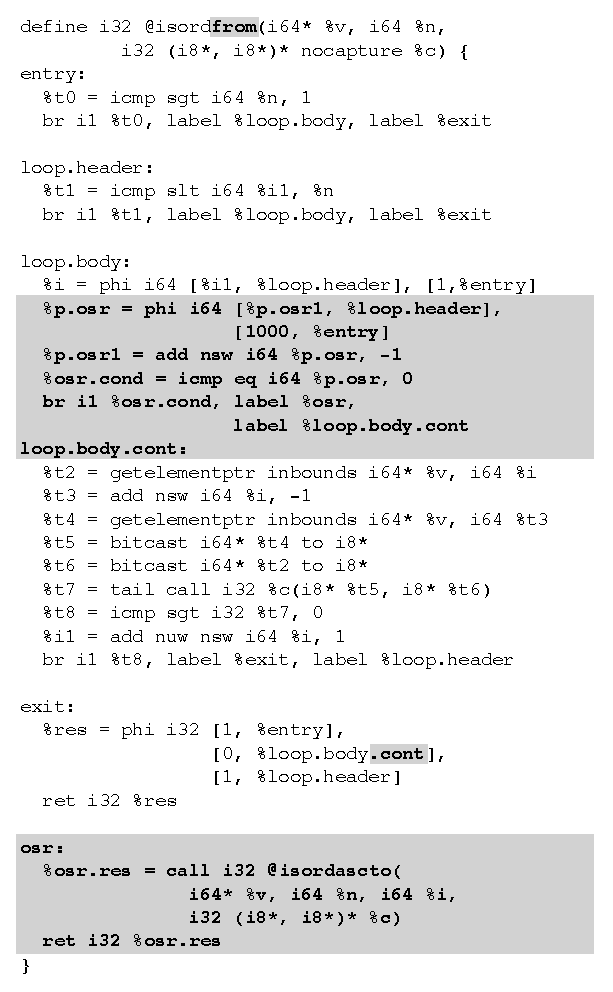
\includegraphics[width=0.9\columnwidth]{figures/isordfrom/isordfrom.eps}
\caption{\protect\label{fig:isordfrom} IR version of base function {\tt isord} (\myfigure\ref{fi:isord-example}) instrumented for resolved OSR. The OSR is fired at the beginning of the loop body after 1000 iterations. Additions resulting from the instrumentation are in grey.
}
\end{center}
\end{figure}
\fi

\ifdefined\noauthorea
\begin{figure}[t]
\begin{center}
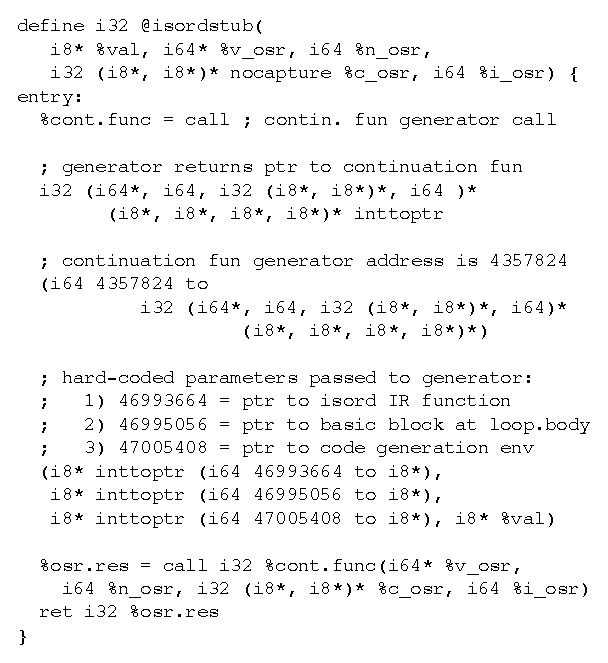
\includegraphics[width=0.9\columnwidth]{figures/isordstub/isordstub.eps}
\caption{\protect\label{fig:isordstub} IR stub that generates the continuation function when an open OSR is fired by {\tt isordfrom} (\myfigure\ref{fig:isordfrom}).
}
\end{center}
\end{figure}
\fi

\ifdefined\noauthorea
\begin{figure}[t]
\begin{center}
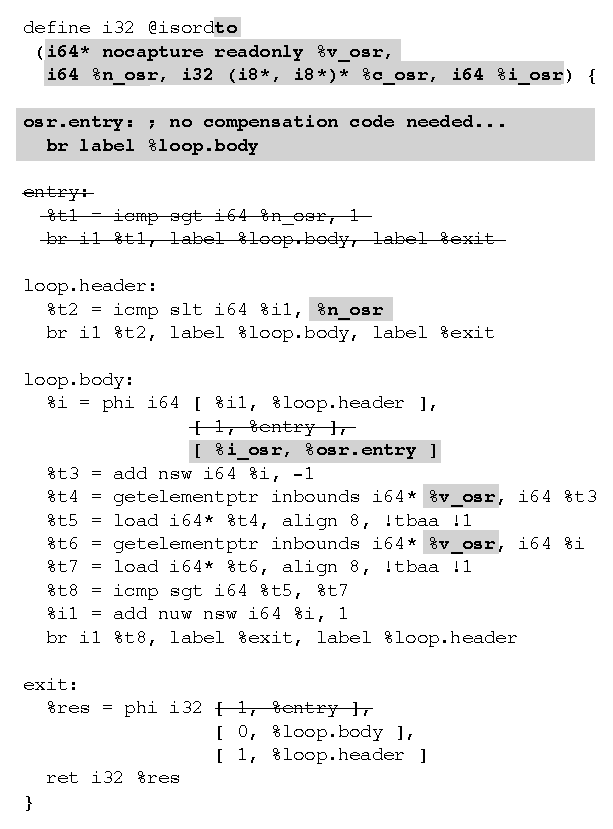
\includegraphics[width=0.9\columnwidth]{figures/isordascto/isordascto.eps}
\caption{\protect\label{fig:isordascto} OSR instrumentation (in grey) of faster variant {\tt isordasc} (\myfigure\ref{fi:osr-dynamics}) in LLVM IR. The original function entry block is unreachable after instrumentation and eliminated (struck-through code fragments).
}
\end{center}
\end{figure}
\fi

\paragraph{OSR Instrumentation in IR.}
To defer the compilation of the continuation function until the comparator is known at run time, we used \osrkit\ to instrument {\tt isord} with an open OSR point at the beginning of the loop body, as shown in \myfigure\ref{fig:isordfrom}. Portions added to the original code by OSR istrumentation are highlighted in grey.
%The figure illustrates how the original {\tt isord} code is instrumented by \tinyvm, highlighting in grey the added portions. 
New instructions are placed at the beginning of the loop body to increments a hotness counter {\tt p.osr} and jump to an OSR-firing block if the counter reaches the threshold (1000 iterations in this example). The OSR block contains a tail call to the target generation stub, which receives as parameters the four live variables at the OSR point ({\tt v}, {\tt n}, {\tt i}, {\tt c}). \osrkit\ allows the stub to receive the run-time value {\tt val} of an IR object that can be used to produce the continuation function -- in our example, the pointer to the comparator function to be inlined. The stub (see \myfigure\ref{fig:isordstub}) calls a code generator that: 1) builds an optimized version of {\tt isord} by inlining the comparator, and 2) uses it to create the continuation function {\tt isordto} shown in \myfigure\ref{fig:isordascto}. The stub passes to the code generator four parameters: 1) a pointer to the {\tt isord} IR code, 2) a pointer to the basic block in {\tt isord} from which the OSR is fired, 3) a user-defined object to support code generation in MCJIT, and 4) the stub's {\tt val} parameter (the first three are hard-wired by \osrkit). The stub terminates with a tail call to {\tt isordto}. To generate the continuation function from the optimized version created by the inliner, \osrkit\ replaces the function entry point, removes dead code, replaces live variables with the function parameters, and fixes $\phi$-nodes accordingly. Additions resulting from the IR instrumentation are in grey, while removals are struck-through.

\ifdefined\noauthorea
\begin{figure}[t]
\begin{center}
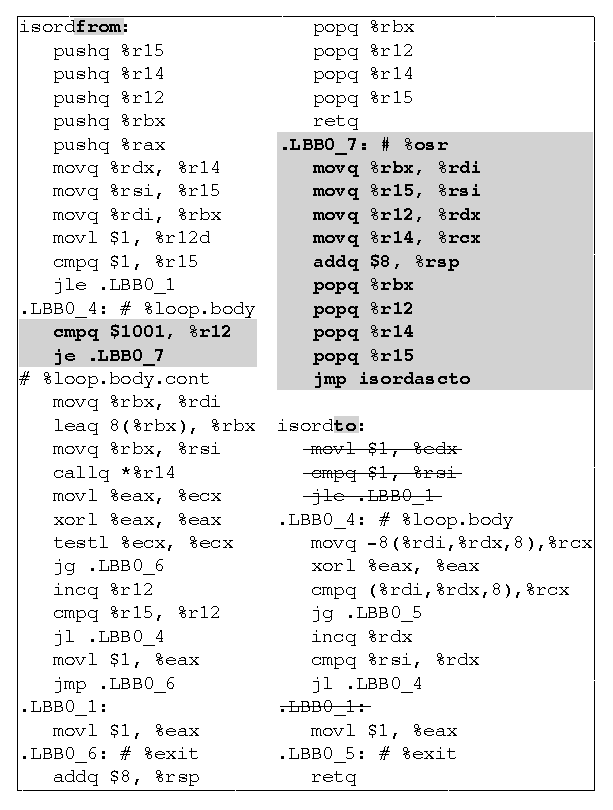
\includegraphics[width=0.9\columnwidth]{figures/isordx86-64/isordx86-64.eps}
\caption{\protect\label{fig:isordx86-64} OSR-instrumented functions {\tt isordfrom} (base) and {\tt isordascto} (faster continuation) after IR to x86-64 lowering in LLVM. For the sake of comparison with the native code that would be generated for the original non-OSR versions, additions resulting from the IR instrumentation are in grey, while removals are struck-through.}
\end{center}
\end{figure}
\fi

\paragraph{x86-64 Lowering.}
\label{se:ir-x86-lowering}

%The final step to be performed before execution is native code generation. 
\myfigure\ref{fig:isordx86-64} shows the x86-64 code generated by the LLVM back-end for {\tt isordfrom} and {\tt isordto}. For the sake of comparison with the native code that would be generated for the original non-OSR versions, additions resulting from the IR instrumentation are in grey, while removals are struck-through. Notice that the OSR intrusiveness in {\tt isordfrom} is minimal, consisting of just two assembly instructions with register and immediate operands. As a result of induction variable canonicalization in the LLVM back-end, loop index {\tt i} and hotness counter {\tt p.osr} are fused in register {\tt\%r12}. We also note that tail call optimization is applied in the OSR-firing block, resulting in no stack growth during an OSR. The continuation function {\tt isordto} is identical to the optimized version of {\tt isord}, except that the loop index is passed as a parameter in {\tt \%rdx} and no loop pre-header is needed since OSR jumps directly in the loop body.

%\subsection{\osrkit\ Instrumentation API}
%\label{se:instrum-api}
%To support the IR instrumentation tasks of \mysection\ref{se:overview}, \osrkit\ provides a number of abstractions for VM builders. 

%In this section we discuss an LLVM implementation of the approach described in \mysection\ref{se:overview}. Our discussion is based on a set of abstractions to support OSR instrumentation of IR code, which we organized in an LLVM-based library for VM builders called \osrkit. A simplified overview of the main building blocks is:
%\begin{itemize}
%\item {\em StateMapper}: a class that [...]
%\item {\em InsertResolvedOSR(f1, b1, f2, b2, cond, m)}: function that inserts a resolved OSR point in function {\em f1} at basic block {\em b1} to function {\em f2} at basic block {\em b2}, using as OSR condition a sequence of IR instructions {\em cond} and a state mapper {\em m}.
%\item {\em InsertOpenOSR()}: [...]
%\item {\em GenerateOSRContFun(...)}: generates the continuation function [...]
%\end{itemize}

%LLVMContext& Context, OSRLibrary::OpenOSRInfo& info,
%        OSRLibrary::OSRCond& cond, Value* profDataVal, OSRLibrary::DestFunGenerator destFunGenerator,
%        std::vector<Value*> *valuesToTransfer, OSRLibrary::OSRPointConfig &config
%Function* src, BasicBlock* src_bb, std::string* F1NewName, OSRLibrary::OSRCond &cond, int branchTakenProb

%The generated stub calls a function inliner that generates a version of {\tt isord} where the comparator's body, pointed to by live variable {\tt c_osr}, is inlined in the loop body. The optimized version {\tt isordto} is shown in \myfigure\ref{fig:isordascto}.

\section{Case Study}
\label{case-study}

MATLAB is a popular dynamic language for scientific and numerical programming. Introduced in the late 1970s mainly as a scripting language for performing computations through efficient libraries, it has evolved over the years into a more complex programming language with support for high-level features such as functions, packages and object orientation. A popular feature of the language is the \feval\ construct, a built-in higher-order function that enable the invocation of the function passed as first argument on the set of subsequent arguments of the {\tt feval} call, and to return the computed result. This feature is heavily used in many classes of numerical computations, such as iterative methods for the approximation of the solutions of ordinary differential equations and simulated annealing heuristics to locate a good approximation to the global optimum of a function in a large search space.

A previous study by Lameed and Hendren~\cite{lameed2013feval} shows that the overhead of an {\tt feval} call is significantly high compared to a direct call, especially in JIT-based execution environments such as McVM and the proprietary MATLAB JIT accelerator by Mathworks. The main reason for this overhead is that the presence of an {\tt feval} instruction can disrupt the results of intra- and inter-procedural level for type and array shape inference analyses, which are a key ingredient for efficient code generation.

Lameed and Hendren thus propose and implement in McVM two dynamic techniques for optimizing {\tt feval} instructions. The first technique is based on OSR: using the McOSR library~\cite{lameed2013modular}, {\tt feval} calls inside loops are instrumented with an OSR point and with profiling code to cache the last-known types for the arguments of each {\tt feval} instruction. When an OSR is fired at run-time, a code generator modifies the original function by inserting a guard to choose between a fast path containing a direct call and a slow path with the original {\tt feval} call. The second technique is less general and uses value-based JIT compilation: when the first argument of an {\tt feval} call is an argument of the enclosing function, the compiler replaces each call to this function in all of its callers with a call to a special dispatcher. When the program is executed, the dispatcher will evaluate the value of the parameter for the {\tt feval} and execute either a previously compiled cached code or generate and JIT-compile a method optimized for the current value of the argument.

Although the OSR-based approach is more general, it generates much less efficient code compared to the JIT-based version for three reasons:
\begin{enumerate}
\item since the function called through {\tt feval} is unknown at compile time, the type inference engine is unable to infer types for the returned values, so the compiler has to generate generic instructions (suitable for handling different types) for the remainder of the code;
\item guard computation is expensive, because not only the value of the first argument, but also the types of the remaining arguments have to be checked to choose between the fast and the slow path;
\item since an {\tt feval} is executed through the interpreter, in the original functions arguments are boxed to make them more generic before the call.
\end{enumerate}

The first one in particular is a major source of inefficiency for the OSR-based approach, since the benefits from replacing the call to the interpreter's {\tt feval} dispatcher with a direct call are limited compared to the optimization opportunities deriving from a better type inference on the whole body of the function. In fact, as they operate on boxed values, instructions operating on generic-type variables are inherently much less efficient than their counterparts for [arrays of] primitive types. While the JIT-based approach is preferable as it generates much better code, on the other hand it cannot be applied to cases in which the first argument $f$ to {\tt feval} is not passed as argument to the enclosing function $g$. Some possible scenarios are:
\begin{itemize}
\item $f$ is an {\tt inline} or an anonymous function defined in $g$;
\item $f$ is the return value from a previous call in $g$ to another function;
%\item $f$ is retrieved from a data structure~\cite{lameed2013feval};
\item $f$ is a constant string containing the name of a user-defined function (a typical inappropriate use of {\tt feval} according to~\cite{radpour2013refactoring}).
\end{itemize}
 
Lameed and Hendren conclude their paper by stating, ``It would be interesting to look at future work that combine the
strengths of both approaches". In the remaining part of this section, we extend McVM by implementing a novel optimization mechanism for {\tt feval} based on our OSR technique: we will show that our mechanism is as efficient as their JIT-based approach in terms of quality of generated code, and is even more general than their OSR-based approach, as it can optimize also {\tt feval} calls not enclosed in a loop.

\subsection{Extending McVM}
The McVM virtual machine is a complex research project developed at McGill and composed of several software components, including: a front-end for lowering MATLAB programs to an intermediate representation called IIR that captures all of the high-level features of the language; an interpreter for running MATLAB functions and scripts in IIR format; a manager component to perform analyses on IIR; a JIT compiler based on LLVM for generating native code for a function, thus lowering McVM IIR to LLVM IR; a set of helper components to perform fast vector and matrix operations using optimized libraries such as ATLAS, BLAS and LAPACK. The architecture of McVM is illustrated in Figure [...]

McVM implements a function versioning mechanism based on type specialization: for each IIR representation of a function, different IR versions are generated according to the types of the arguments at each call site. The number of generated versions per function is on average small (i.e., less than two), as in most cases functions are always called with the same argument types. Type specialization is the main factor for the generation of efficient code in McVM~\cite{chevalier2010mcvm}.

The source code of McVM is publicly available~\cite{mcvm}, and after porting it from the legacy LLVM JIT to MCJIT, we have extended it with the following components to enable the optimization of {\tt feval} instructions:
\begin{enumerate}
\item An analysis pass for {\tt feval} instructions in the IIR representation of a function
\item An extension for the IIR compiler to track the correspondence between IIR and IR objects at {\tt feval} calls
\item A helper component to insert OSR points in the IR at IIR locations annotated during the analysis pass
\item A callback optimizer triggered at OSR points, which in turn is made of:
\begin{enumerate}
\item A profile-driven IIR generator to replace {\tt feval} calls with direct calls
\item A helper component to lower the optimized IIR function to IR and construct a state mapping 
\item A code caching mechanism to handle the compilation of the continuation functions
\end{enumerate}
\end{enumerate}

The analysis pass is integrated in McVM's analysis manager and identifies optimization opportunities for functions containing {\tt feval} instructions. A function becomes a candidate for optimization when at least one of its {\tt feval} calls is inside a loop. We then group {\tt feval} instructions whose first argument is reached by the same definition, using reaching definition information already computed by the analysis manager for previous optimizations. For each group we mark for instrumentation only those instructions that dominate the others, so that the function can be optimized as early as possible at run-time.

The analysis pass is also able to determine whether the value of the argument can change across two executions of the same {\tt feval} instruction, thus discriminating when a run-time guard must be inserted during the run-time optimization phase. Compared to the OSR-based approach by Lameed and Hendren, our solution is cheaper because the types for the other arguments do not need to be cached or guarded: as we will see later, the type inference engine will compute the most accurate yet sound type information in the analysis of the optimized IIR where direct calls are used.

When the IIR compiler processes an annotated {\tt feval} instruction, it will store in the metadata of the function version being compiled a copy of its variable map (i.e., a map between IIR and IR objects), the current {\tt llvm::BasicBlock*} created for the call and the {\tt llvm::Value*} object corresponding to the first argument for the {\tt feval}. The last two objects are used by the helper component as source label and profiling value for inserting an open OSR point, with the copy of the variable map being passed (along with other information) as {\tt extra} field. The open-OSR stub will in turn invoke the callback optimizer component we are about to describe in the next subsection.

\subsection{Generating optimized code}
The core of the optimization pipeline is the callback optimizer component, that is responsible for generating optimized code for the current function $f$ using profiling (i.e., the object containing the first argument for \feval\) and contextual information passed from the open-OSR stub. As a first step, the optimizer will process the profiling object to resolve the target of the call, which we call $g$. 
%TODO dire del code caching
A new function $f_{OSR}$ is then generated by cloning the IIR representation $f^{IIR}$ of $f$ into $f^{IIR}_{OSR}$ and replacing all the \feval\ calls in the same group of the instrumented one with direct calls to $g$.

As a next step, the optimizer asks the IIR compiler to generate IR code for $f^{IIR}_{OSR}$, also saving a copy of the variable map when compiling the direct call corresponding to the \feval\ instruction that triggered the OSR transition. This variable map is compared against the variable map stored during the lowering phase for $f$ 
  
  
  
  
  
  
  
  
  
  
\section{Experimental Evaluation}
\label{se:experiments}

In this section we present a preliminar experimental study of our OSR technique in TinyVM, a proof-of-concept virtual machine based on LLVM's JIT compiler MCJIT. TinyVM supports interactive invocations of functions and it can compile LLVM IR either generated at run-time or loaded from disk. The main design goal behind TinyVM is the creation of an interactive environment for IR manipulation and JIT-compilation of functions: for instance, it allows the user to insert OSR points in loaded functions, run optimization passes on them or display their CFGs, repeatedly invoke a function for a specified amount of times and so on. TinyVM supports dynamic library loading and linking, and comes with a helper component for MCJIT that simplifies tasks such as handling multiple IR modules, symbol resolution in presence of multiple versions of a function, and tracking native code and other machine-level generated object such as Stackmaps.

TinyVM is thus an ideal playground to exercise our OSR technique, and we use it to run performance measurements on the shootout test suite, also known as the Computer Language Benchmark Game~\cite{shootout}. The list of benchmarks and their description is reported in Table [...].

\subsection{Setup}

We generated the IR modules for our experiments with clang, starting from the C version of the shootout suite. No LLVM optimization passes were performed on the code other than {\em mem2reg}, which promotes memory references to be register references and is typically used in SSA form construction.

\subsection{Results}

\begin{itemize}
\item {\bf Message 1}: how much does a never-firing OSR point impact code quality? We run a program with one or more OSR points, and we measure the slowdown given by factors such as cache effects (due to code bloat), register pressure, etc. due to the presence of the OSR points.
\item {\bf Message 2}: what is the overhead of an OSR transition to the same function? We run a program with a controlled OSR transition, e.g., with a counter that fires the OSR. Here we measure the impact of the actual OSR call [we already tried this with the repeated addition microbenchmark simple\_loop\_SSA.ll].
\item {\bf Message 3}: what is the overhead of the library for inserting OSR points?
\end{itemize}

\paragraph{Impact on code quality}
In order to measure how much a never-firing OSR point might impact code quality, we analyzed the source-code structure of each benchmark and profiled its run-time behavior to identify performance-critical sections for OSR point insertion.

For iterative benchmarks, we insert an OSR point in the body of their hottest loops. We classify a loop as hottest when its body is executed for a very high cumulative number of iterations (e.g., from a few thousands up to billions) and it either calls the method with the highest {\em self} time in the program, or it performs the most computational-intensive operations for the program in its own body. These loops are natural candidates for OSR point insertion, as they can be used - as in the Jikes RVM - to enable more dynamic inlining opportunities, with the benefits from several control-flow (e.g., dead code elimination) and data-flow (e.g., constant propagation) optimizations based on the run-time values of the live variables. In the shootout benchmarks, the number of such loops is typically 1 (2 for {\tt spectral-norm}).

For recursive benchmarks, we insert an OSR point in the body of the method that accounts for the largest {\em self} execution time of the program. Such an OSR point might enable recompilation of the invoked method at a higher degree of optimization, [...]

In the shootout benchmarks, ({\tt binary-trees} and {\tt spectral-norm}) show a recursive pattern.
  
  
  
  
  
  
  
  
  
  
  
  
\section{Related Work}
\label{se:related}

\paragraph{Early Approaches.}
%OSR has been pioneered in the SELF language~\cite{holzle1992self} to enable source-level debugging of optimized code, which required deoptimizing the code back to the original version. To reconstruct the source-level state, the compiler generates {\em scope descriptors} recording for each scope the locations or values of its arguments and locals. Execution can be interrupted only at certain interrupt points (i.e., method prologues and backward branches in loops) where its state is guaranteed to be consistent, allowing optimizations between interrupt points. It is worth mentioning also the {\em deferred compilation} mechanism~\cite{chambers1991self} implemented in SELF for branches that are unlikely to occur at run-time: the system generates a stub which invokes the compiler to generate a code object that can reuse the stack frame of the original code.

OSR has been pioneered in the SELF language~\cite{holzle1992self} to enable source-level debugging of optimized code, which required deoptimizing the code back to the original version. To reconstruct the source-level state, the compiler generates {\em scope descriptors} recording locations or values of arguments and locals. Execution can be interrupted only at certain interrupt points where its state is guaranteed to be consistent (i.e., method prologues and backward branches in loops), allowing optimizations between interrupt points. SELF also implements a deferred compilation mechanism~\cite{chambers1991self} for branches that are unlikely to occur at run-time: the system generates a stub which invokes the compiler to generate a code object that can reuse the stack frame of the original code.

\paragraph{Java Virtual Machines.}
The success of the Java language has drawn more attention to the design and implementation of OSR techniques, as bytecode interpreters began to work along with JIT compilers. In the high-performance HotSpot Server JVM~\cite{paleczny2001hotspot} performance-critical methods are identified using method-entry and backward-branches counters; when the OSR threshold is reached, the runtime transfers the execution from the interpreter frame to an OSR frame and the compiled code. Deoptimization is performed when class loading invalidates inlining or other optimization decisions: execution is rolled forward to a safe point, at which the native frame is converted into an interpreter frame.

\ifdefined \fullver
Whaley~\cite{whaley2001osr} proposes a technique to identify intra-method code regions that are rarely executed, and thus compile and optimize the code without these regions. A rare block is replaced by a stub that transfers the control to the interpreter, while a glue routine reconstructs the state from the interpreter starting from a table storing the location, in registers or memory, of each variable in the original bytecode.
\fi

The Jikes RVM uses an OSR mechanism~\cite{fink2003design} that extracts a scope descriptor from a thread suspended at a method's entrypoint or backward branch, creates specialized code to setup the stack frame for the optimized compiled code and resumes the execution at the desired program counter. OSR is used as part of an automatic, online, profile-driven deferred compilation mechanism.
\ifdefined \fullver
A more general approach has then been proposed in~\cite{soman2006efficient}, with the OSR implementation decoupled from program code to ease more aggressive specializations triggered by events external to the executing code (e.g. class loading, exception conditions). Execution state information is maintained in a variable map - a per-method list of thread-switch points and associated live bytecode variables - that is incrementally updated across a wide range of basic compiler optimizations.
\else
A more general solution is proposed in~\cite{soman2006efficient}, with the OSR implementation decoupled from program code to ease more aggressive specializations triggered by events external to the executing code (e.g., class loading). Execution state information is maintained in a variable map that is incrementally updated across a wide range of basic compiler optimizations.
\fi

\ifdefined \fullver
In the Graal VM - a modified version of HotSpot centered on the principle of speculative optimizations - the execution falls back to the interpreter during deoptimization, while a runtime function restores the stack frames in the interpreter using the metadata associated with the deoptimization point~\cite{duboscq2013graal,wurthinger2013truffle,duboscq2014metadata}.
\else
In the Graal VM, which is centered on the principle of speculative optimizations, the execution falls back to the interpreter during deoptimization, while a runtime function restores the stack frames in the interpreter using the metadata associated with the deoptimization point~\cite{duboscq2013graal,wurthinger2013truffle,duboscq2014metadata}.
\fi

% TODO only if we have space: HotpathVM

\paragraph{Prospect.} Prospect~\cite{susskraut2010prospect} is an LLVM-based framework for parallelizing a sequential application. The IR is instrumented through two LLVM passes to enable switching at run-time between a slow and a fast variant of the code, which are both compiled statically. Helper methods are used to save and eventually restore registers, while stack-local variables are put on a separate {\tt alloca} stack rather than on the stack frame so that the two variants result into similar and thus interchangeable stack layouts.
\ifdefined \fullver
Speculative variables~\cite{susskraut2009speculation} are introduced when the slow variant needs to track state (e.g., information for out-of-bound checks) that is missing in the fast variant. Switching operations are performed by Prospect at user-specified checkpoints in the original code.
\fi

\paragraph{McOSR.} McOSR~\cite{lameed2013modular} is a library for the LLVM legacy JIT compiler to insert OSR points at loop headers. When an OSR transition is fired, the live state is saved into a set of global variables (one per live variable) and a helper method is invoked to modify the IR of the function using a code transformer provided by the front-end and a copy of the original code saved as control version. The library generates a new entrypoint for the function to check a global condition and discriminate whether the function is being invoked through an OSR transition or a regular call: in the first case, values for live variables are read from the associated global variables, and the execution jumps to the block to resume the execution at.
\ifdefined \fullver
The SSAUpdater component of LLVM is then used to restore the SSA form after the update.
\fi
When the helper method returns, the updated function is invoked and the OSR is thus performed in a new stack frame. When the updated function returns, a second helper method is called to recompile the updated function to remove the new entrypoint inserted for the OSR transition, as it can disrupt LLVM optimizations and lead to poorer performance on subsequent invocations of the function.

\paragraph{Other Related Work.}
\ifdefined \fullver
Dynamic Software Updating (DSU) is a methodology for permitting programs to be updated while they run and is thus useful for systems that cannot afford to halt service. DSU techniques (e.g. ~\cite{neamtiu2006dsu,makris2009dsu}) are required to update all functions active on the call stack at the same time, so their code should be instrumented and data types wrapped to support future extensions.

\fi
In tracing JIT compilers deoptimization techniques are used to safely leave an optimized trace when a guard fails and to continue the execution in the interpreter or with a different piece of code. SPUR~\cite{bebenita2010spur} is a trace-based JIT compiler for Microsoft's Common Intermediate Language (CIL) with four levels of JIT-ting: profiling, tracing, optimizing and transfer-tail; transfer-tail JIT is used to bridge the execution from an instruction in a block from tracing or optimizing mode to the next safe point for deoptimization to profiling code. In RPython guards are implemented as a conditional jump to a trampoline that analyzes resume information for the guard and executes compensation code to leave the trace; resume data is compactly encoded by sharing parts of the data structure between subsequent guards~\cite{schneider2012rpython}. A similar approach is used in LuaJIT, where sparse snapshots are taken to enable state restoration when leaving a trace~\cite{luajit}.

% TODO: speculative parallelization? (e.g. FastTrack)

%\cite{detlefs2001method,steiner2007adaptive,chambers1992design}
 % !TEX root = article.tex

\section{Conclusions}
\label{se:conclusions}

In this paper, we have presented an OSR framework that introduces novel ideas and combines features of extant techniques that no previous solution provided simultaneously. Relevant aspects include platform independence~\cite{lameed2013modular}, generation of highly optimized continuation functions~\cite{fink2003design}, and performing deoptimization without the need for an interpreter~\cite{bebenita2010spur}. Two novel features we propose are OSR with compensation code, which allows to extend the range of points where OSR transitions can be fired, and the ability to inject OSR points at arbitrary locations. Using these features, we have shown how to improve the state of the art of \feval\ optimization in MATLAB virtual machines. We have also investigated the feasibility of our approach in LLVM, showing that it is efficient in practice.

%\ifx\noauthorea\undefined
\paragraph{Acknowledgements.}

We wish to thank Jan Vitek, Petr Maj, Karl Millar, and Olivier Fl{\"u}ckiger for many enlightening discussions. We are especially grateful to Jan for sparking our interest in this exciting line of research. % during a pleasant visit at Purdue University and for interesting conversations in many other occasions.
%\fi

\paragraph{Live Version of this Paper.}
We complement the traditional scholarly article publication model by maintaining a live version of this paper at \url{https://www.authorea.com/users/55853/articles/66046}. The live version incorporates continuous feedback by the community, providing post-publication fixes, improvements, and extensions.


%\appendix
%\section{Appendix Title}

%This is the text of the appendix, if you need one.

%\acks

%Acknowledgments, if needed.

% We recommend abbrvnat bibliography style.

\bibliographystyle{abbrvshortnat}
\bibliography{bibliography/biblio.bib}
%\AtEveryBibitem{\clearlist{language}} % clears language
%\AtEveryBibitem{\clearfield{note}}    % clears notes

\end{document}

%                       Revision History
%                       -------- -------
%  Date         Person  Ver.    Change
%  ----         ------  ----    ------

%  2013.06.29   TU      0.1--4  comments on permission/copyright notices

